\providecommand{\topdir}{..}
\documentclass[../main.tex]{subfiles}

\externaldocument{\subfix{../00_front_matter/front_matter}}
\externaldocument{\subfix{../01_introduction/introduction}}
\externaldocument{\subfix{../02_lorenz96/lorenz96}}
\externaldocument{\subfix{../03_rayleigh_benard/rayleigh_benard}}
\externaldocument{\subfix{../04_tendencies/tendencies}}
\externaldocument{\subfix{../05_evaluation/evaluation}}
\externaldocument{\subfix{../06_conclusion/conclusion}}

\begin{document}

\ifSubfilesClassLoaded{
    \frontmatter
    \tableofcontents
    \mainmatter
}{}

\appendix
\chapter{Description of codebase and data} \label{chap:computations}
\epigraphhead[0.1\textheight]{
    \epigraph{\todo{epigraph}}{}
}

\section{Reproducibility}
% cite reproducibility paper!


\chapter{Details of numerical experiments} \label{chap:details}
% \setlength{\epigraphwidth}{.45\textwidth}
\epigraphhead[0.1\textheight]{
    \epigraph{\todo{epigraph}}{}
}


\section{Initial condition} \label{sec:initial_condition}
The initial velocity field is specified in terms of the streamfunction
(whose level curves are streamlines of the flow)
\[
    \psi_0(x, z) = 0.1 \sin(\pi x) (1 - (2z - 1)^2)^2,
\]
from which
\[
    u_0(x, z) = -\pdiff{\psi_0}{z}
    \quad \text{and} \quad
    w_0(x, z) = \pdiff{\psi_0}{x}.
\]
It is easily verified that these satisfy the required boundary conditions. The
reason for using the streamfunction is that it guarantees a divergence-free
velocity field ($\partial u /\partial x + \partial w /\partial z = -\partial^2
\psi/\partial x \partial z + \partial^2 \psi/\partial z \partial x \equiv 0$).

The initial temperature field is
\[
    \theta_0(x, z) = \frac{1}{2} (1 - 2z)^9
\]
plus a random perturbation at each grid point, drawn from the normal
distribution with mean zero and height-dependent standard deviation
$(1 - (2z - 1)^2) \times 10^{-2}$. The random perturbation is necessary to
break the symmetry that the initial condition would otherwise have.

\cref{fig:init} shows the initial streamfunction, velocity and temperature
fields. There are eight equally-sized counter-rotating convection cells.

\begin{figure}[ht]
    \centering
    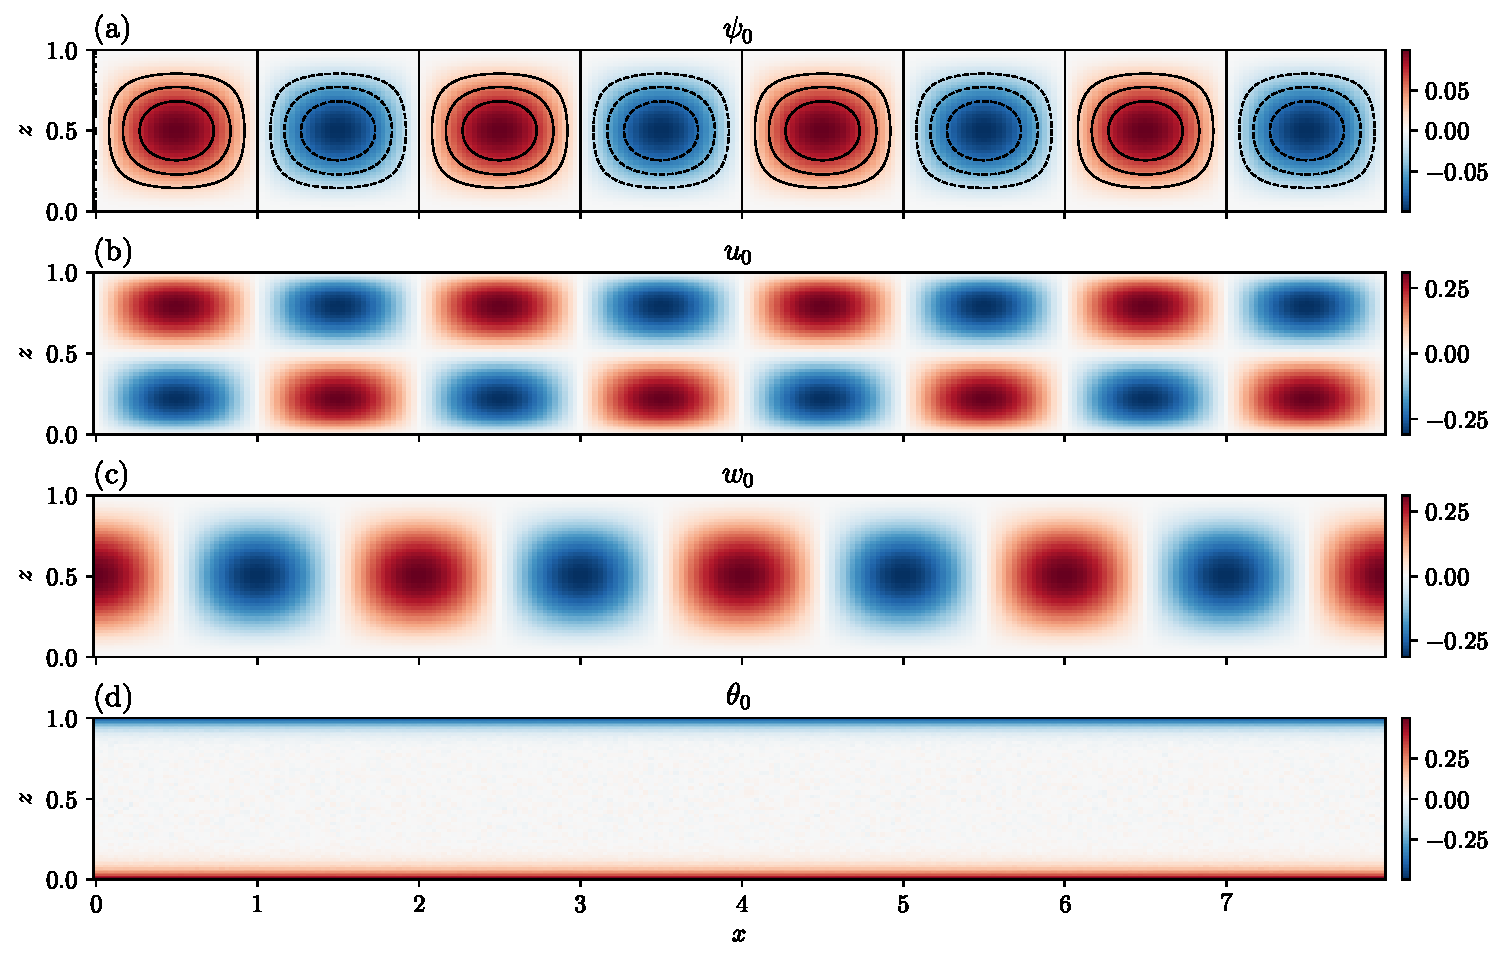
\includegraphics[width=\linewidth]{figures/init.pdf}
    \caption{
        Initial streamfunction \textbf{(a)}, horizontal velocity \textbf{(b)},
        vertical velocity \textbf{(c)} and temperature \textbf{(d)}.
    }
    \label{fig:init}
\end{figure}


\section{Model spin-up time} \label{sec:spinup}
It is critical to ensure that the simulations have reached a statistically
steady state (to ``spin'' them up) in order to accurately calculate long-term
statistics. To that end, I have calculated the 250-time-unit rolling means of
the Nusselt number, thermal boundary layer thickness, RMS speed, kinetic energy
dissipation rate and thermal dissipation rate (see
\cref{sec:choose_resolution} for the definitions) using the data from the
$1024 \times 128$ simulation described in \cref{sec:choose_resolution}.
These are plotted in \cref{fig:1024x128_spin_up}. The RMS speed and kinetic
energy dissipation rate take longer than the other variables to reach a steady
state and exhibit larger low-frequency oscillations. Nonetheless, I determine
that the simulation has reached a sufficiently steady state at $t = 750$.

\begin{figure}[ht]
    \centering
    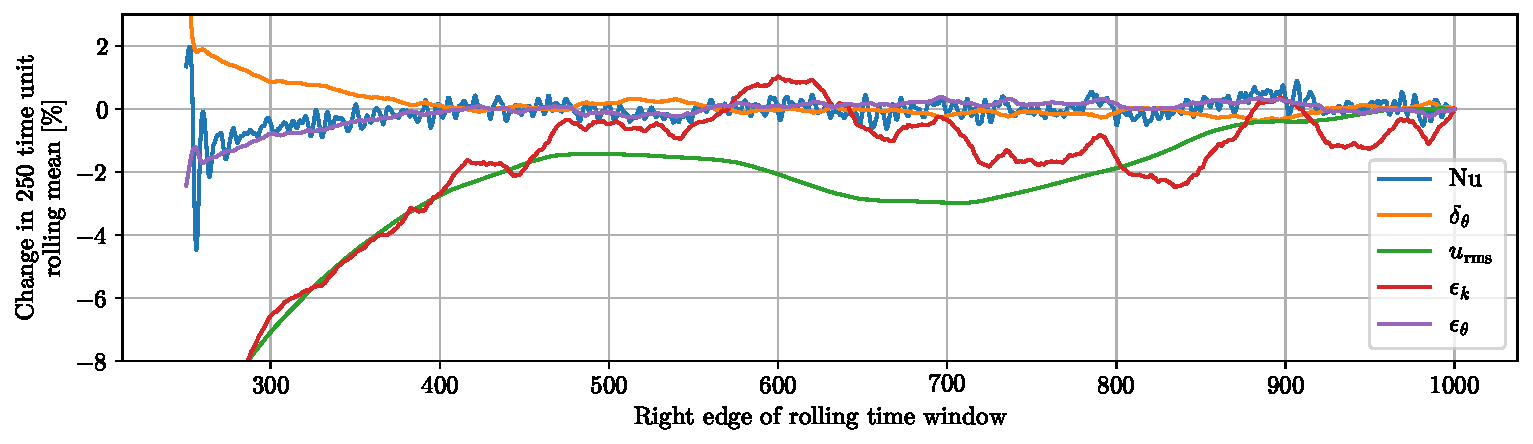
\includegraphics[width=\linewidth]{figures/1024x128_spin_up.pdf}
    \caption{
        250-time-unit rolling means of the Nusselt number $\nusselt$, thermal
        boundary layer thickness $\delta_\theta$, RMS speed $u_\mathrm{rms}$,
        kinetic energy dissipation rate $\epsilon_k$ and thermal dissipation
        rate $\epsilon_\theta$ for the $1024 \times 128$ simulation described
        in \cref{sec:choose_resolution}. The horizontal coordinate is the
        position of the \emph{right} edge of the rolling window. Each quantity
        is expressed as a percentage deviation relative to its value when
        the right edge of the window is at $t=1000$.
    }
    \label{fig:1024x128_spin_up}
\end{figure}

In the resolution-dependence experiment of \cref{sec:choose_resolution}, the
simulations with resolution higher than $1024 \times 128$ were initialised by
interpolating the $1024 \times 128$ solution at time $t = 650$. These also
needed to reach a statistically steady state. \cref{fig:2048x256_spin_up} shows
the 150-time-unit rolling means of the same quantities as
\cref{fig:1024x128_spin_up} for the $2048 \times 256$ simulation. I determine
that the means reach a sufficiently steady state when the right edge of the
rolling window is at $t=900$; it is therefore appropriate to use the data
from $t=900-150=750$ onwards.
\begin{figure}[ht]
    \centering
    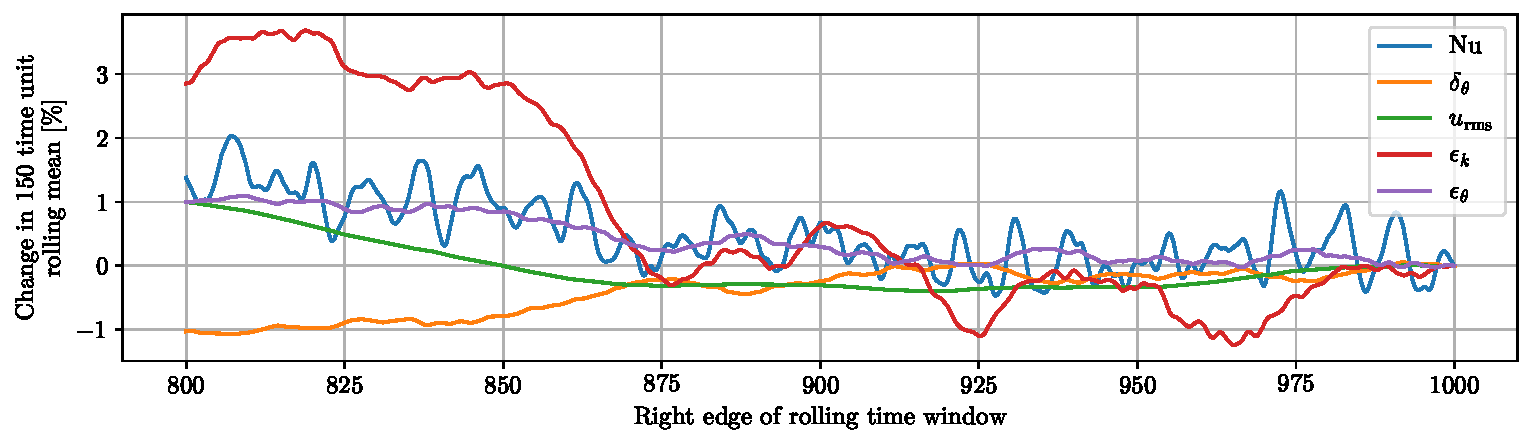
\includegraphics[width=\linewidth]{figures/2048x256_spin_up.pdf}
    \caption{
        Similar to \cref{fig:1024x128_spin_up}, but showing 150-time-unit
        rolling means for the $2048 \times 256$ simulation, which was
        initialised by interpolating the $1024 \times 128$ solution at time
        $t=650$.
    }
    \label{fig:2048x256_spin_up}
\end{figure}

\subsection{Parametrised model spin-up time} \label{sec:parametrised_spinup}
The parametrised model described in \cref{chap:evaluation} was very slow
to reach a statistically steady state. \cref{fig:parametrised_spin_up} performs
the same rolling mean analysis as above with a 250 time unit window;
I determine that 800 time units are required.

\begin{figure}[ht]
    \centering
    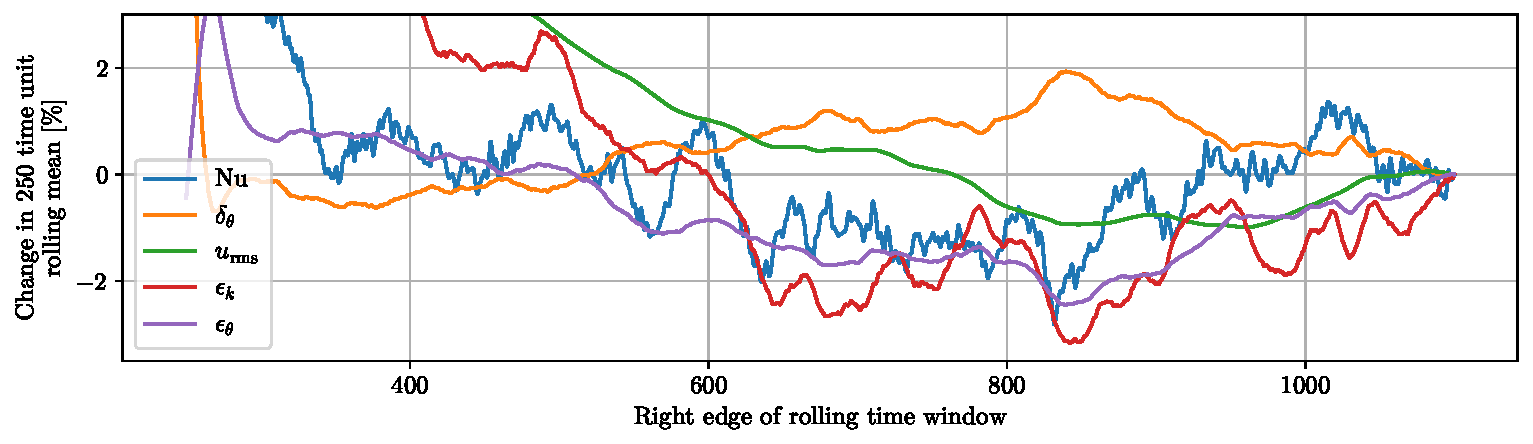
\includegraphics[width=\linewidth]{figures/parametrised_spin_up.pdf}
    \caption{
        Similar to \cref{fig:1024x128_spin_up}, for the parametrised
        $256 \times 64$ simulation.
    }
    \label{fig:parametrised_spin_up}
\end{figure}


\clearpage
\section{Training dataset snapshot frequency} \label{sec:snapshot_freq}
When building the parametrisation training dataset for
\cref{chap:tendencies}, the amount of storage space demanded by the
high-resolution model output made it desirable to avoid saving redundant
information. Saving the model state every time step or every 0.2 time units
(as in \cref{sec:choose_resolution}) would waste space and reduce the
diversity of the training dataset, because the state exhibits substantial
autocorrelation at these intervals. \cref{fig:autocorr} shows the
spatially averaged temporal autocorrelation functions of $u$, $w$ and $\theta$,
computed for the $1024 \times 128$ simulation that is described in
\cref{sec:choose_resolution} (again discarding the first 750 time units of
data for spin-up). Observing that all three variables reach the first
correlation minimum at a lag of approximately 3 time units, I choose to
save the model output at this interval.

\begin{figure}[ht]
    \centering
    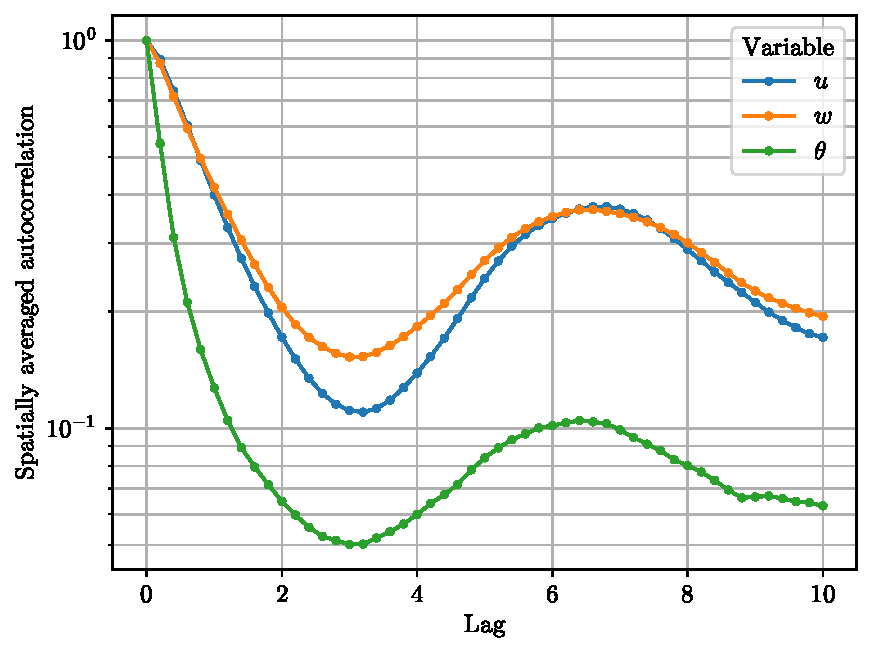
\includegraphics[width=0.6\linewidth]{figures/autocorrelation.pdf}
    \caption{
        Spatially averaged autocorrelation functions of the three prognostic
        variables in the $1024 \times 128$ simulation that is described in
        \cref{sec:choose_resolution}.
    }
    \label{fig:autocorr}
\end{figure}


\ifSubfilesClassLoaded{%
    \emergencystretch=5em
    \printbibliography{}
}{}

\end{document}
